\mcmSection{模型的建立与求解}

\mcmSubsection{问题1:通过解三角行求出多波束探测的覆盖宽度}

在问题1中,$\alpha$是测垂面与海底坡面的交线与水平面的夹角,实际上正是测坡角。也就是说,在问题一种,存在等式:

\begin{equation}
    \gamma = \alpha
\end{equation}

\begin{figure}[h]
    \centering
    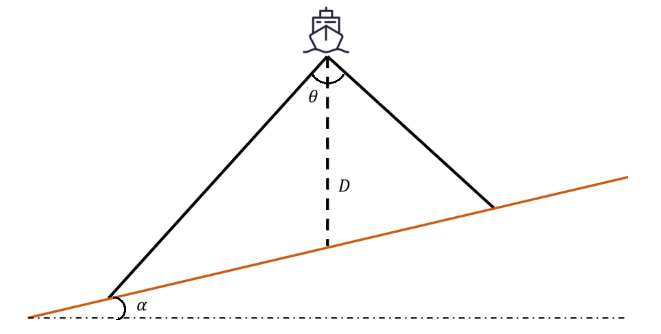
\includegraphics[scale=0.5]{res/img/探测船探测正视图.png}
    \caption{探测船探测正视图}
    \label{fig:探测船探测正视图}
\end{figure}

根据图\ref{fig:探测船探测正视图},为了求出覆盖宽度,可以抽象出如下的几何问题:

已知$\vartriangle PAB$是以$PA$、$PB$为腰的等腰三角形,其中,点$C$是$BP$上任意一点, PM是AB的垂线,且$\angle APB = \theta$, $\angle CAB = \gamma$, $PM = D$(如图\ref{fig:理想情况下的覆盖区域几何图}),求出$AC$在$AB$上的投影。

\begin{figure}[h]
    \centering
    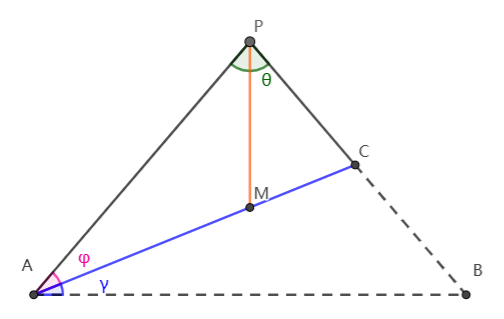
\includegraphics[scale=0.4]{res/img/理想情况下的覆盖区域几何图.png}
    \caption{理想情况下的覆盖区域几何图}
    \label{fig:理想情况下的覆盖区域几何图}
\end{figure}

由题意可设$AM=x_1$,$MC=x_2$,$\angle PAM = \frac{\pi - \theta}{2} - \gamma = \varphi $.

对于$\vartriangle PAM$,根据正弦定理,存在方程:

\begin{equation*}
    \frac{\sin\angle APM}{AM} = \frac{\sin\angle PAM}{PM}
\end{equation*}

对于$\vartriangle PCM$,根据正弦定理,存在方程:

\begin{equation*}
    \frac{\sin\angle CPM}{CM} = \frac{\sin\angle PCM}{PM}
\end{equation*}

综上所述,将对应的值带入方程,可得下列方程组:

\begin{equation}
    \begin{cases}
        \varphi = \frac{\pi - \theta}{2} - \gamma \\
        \frac{\sin \frac{\theta}{2}}{x_1} = \frac{\sin\varphi}{D} \\
        \frac{\sin \frac{\theta}{2}}{x_2} = \frac{\sin(\pi-\theta-\varphi)}{D}
    \end{cases}
\end{equation}

解上述方程组以后,可得:

\begin{equation}
    AC = x_1 + x_2 
       = \frac{\sin\frac{\theta}{2}}{\sin\varphi}D + \frac{\sin\frac{\theta}{2}}{\sin(\varphi - \theta)}D
\end{equation}

综上,可得如下结论:

\textbf{关键结论1:宽度覆盖公式}

探测船的覆盖宽度$W$,与它的多波束换能器的开角$\theta$、测坡角$\gamma$、距离海底的深度$D$有关,满足如下等式:

\begin{equation}
    W = 
    Proj AC = 
    \left(\frac{\sin\frac{\theta}{2}}{\sin\varphi}D + \frac{\sin\frac{\theta}{2}}{\sin(\varphi - \theta)}D\right) \cdot \cos \gamma
    \label{equ:覆盖宽度公式}
\end{equation}

重叠率定义为:

\begin{equation}
    \eta = 1 - \frac{d}{W}
\end{equation}

其中$d$为距离中心点处的距离,$W$为覆盖宽度。

当$\theta = 120^\circ$,$\alpha=\gamma=1.5^\circ$,中心距离$D_0 = 70m$时,带入覆盖宽度公式和重叠率定义,得出下列结果:

% Please add the following required packages to your document preamble:
% \usepackage{booktabs}
\begin{table}[h]
    \centering
    \caption{\textbf{问题1的计算结果}}
    \begin{tabular}{@{}ccllllllll@{}}
    \toprule
    测线距中心点处的距离/$m$  & $-800$ & $-600$ & $-400$ & $-200$ & $0$ & $200$ & $400$ & $600$ & $800$ \\ \midrule
    海水深度/$m$        &      &      &      &      & 70  &     &     &     &     \\
    覆盖宽度/$m$        &      &      &      &      &   &     &     &     &     \\
    与前一条测线的重叠率/$\%$ &   -  &      &      &      &   &     &     &     &     \\ \bottomrule
    \end{tabular}
\end{table}


\mcmSubsection{问题二:一般情况下,覆盖率求解}

根据题意,可以抽象出如下的几何问题:

有两个直三棱柱如图\ref{fig:一般情况下的覆盖区域几何图}所示摆放,三棱柱$BEC-AFD$的侧边与三棱柱$DHC-FGE$的侧边相重合(这里用词是否准确?),其中,$AF$垂直于$FE$,$FG$垂直于$GE$,$\angle AFG=\beta$,$\angle CBE=\alpha$。设平面$ABCD$与平面$HCEG$的交线为$l_s$(图中未画出),求$l_s$与平面$ABEF$的夹角。

\begin{figure}[h]
    \centering
    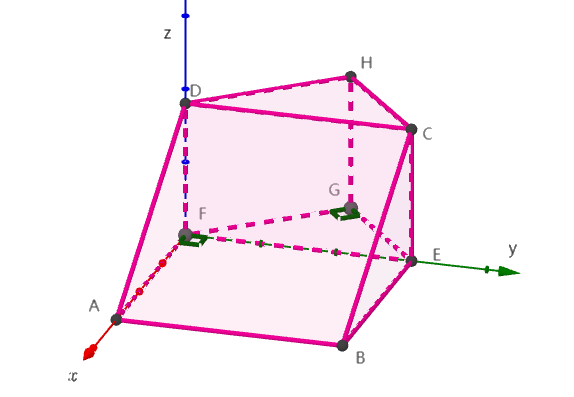
\includegraphics[scale=0.4]{res/img/一般情况下的覆盖区域几何图.png}
    \caption{一般情况下的覆盖区域几何图}
    \label{fig:一般情况下的覆盖区域几何图}
\end{figure}

分别设平面ABCD与平面HCEG的法向量为$\tau_\text{坡}$和$\tau_\text{测}$,$l_s$的方向向量为$v_s = (x_0, y_0, z_0)$.

根据平面法向量的性质,存在方程组:

\begin{equation}
    \begin{cases}
        \tau_\text{坡} \cdot v_s = 0 \\
        \tau_\text{测} \cdot v_s = 0
    \end{cases}
\end{equation}

又因为$\angle AFG=\beta$,$\angle CBE=\alpha$,可得:

\begin{equation}
    \begin{cases}
        \tau_\text{坡} = (\sin\alpha, 0, \cos\alpha) \\
        \tau_\text{测} = (\cos\beta, \sin\beta, 0)
    \end{cases}
\end{equation}

故有方程组:

\begin{equation}
    \begin{cases}
        x_0\sin\alpha + z_0\cos\alpha = 0 \\
        x_0\cos\beta + y_0 \sin\beta = 0
    \end{cases}
\end{equation}

即:

\begin{equation*}
    \begin{cases}
        y_0 = -x_0 \cot \beta \\
        z_0 = -x_0 \tan \alpha
    \end{cases}
\end{equation*}

不妨令$x_0 = -1$,则有:

\begin{equation}
    v_s 
    = (x_0, y_0, z_0)
    = \left( 
            -1,
            \cot \beta,
            \tan \alpha
      \right)
\end{equation}

因而:

\begin{equation*}
    \tan <l_s, ABEF> = \frac {\tan \alpha} {\sqrt{(-1)^2 + \cot ^2 \beta}}
\end{equation*}

所以,$l_s$与平面$ABEF$的夹角为

\begin{equation}
    <l_s, ABEF> = \arctan \left(|\sin \beta| \tan \alpha\right)
\end{equation}

% Please add the following required packages to your document preamble:
% \usepackage{multirow}
\begin{table}[h]
    \centering
    \caption{问题2的计算结果}
    \begin{tabular}{cccccccccc}
    \hline
    \multicolumn{2}{c}{\multirow{2}{*}{覆盖宽度/m}} & \multicolumn{8}{c}{测量船距海域中心点处的距离/海里}        \\ \cline{3-10} 
    \multicolumn{2}{c}{}                        & 0 & 0.3 & 0.6 & 0.9 & 1.2 & 1.5 & 1.8 & 2.1 \\ \hline
    \multirow{8}{*}{测线方向夹角/°}       & 0         &   &     &     &     &     &     &     &     \\
                                    & 45        &   &     &     &     &     &     &     &     \\
                                    & 90        &   &     &     &     &     &     &     &     \\
                                    & 135       &   &     &     &     &     &     &     &     \\
                                    & 180       &   &     &     &     &     &     &     &     \\
                                    & 225       &   &     &     &     &     &     &     &     \\
                                    & 270       &   &     &     &     &     &     &     &     \\
                                    & 315       &   &     &     &     &     &     &     &     \\ \hline
    \end{tabular}
\end{table}

\mcmSubsection{问题三:为海域设计排线方案}

\mcmSubsubsection{方案设计与证明}

\mcmSubsubsection{计算流程}

\mcmSection{模型的评价与改进}